\begin{figure}[h!]
\begin{center}
\centerline{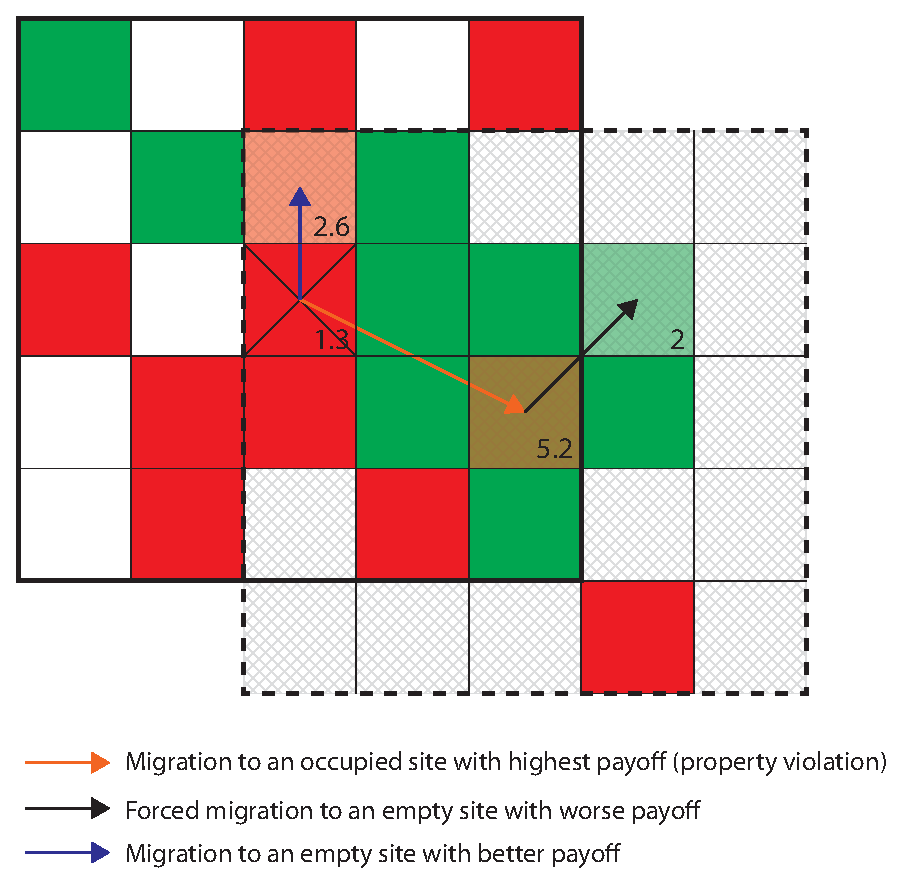
\includegraphics[width=9cm]{../figures2/migration_diagram.eps}}
\caption{Migration diagram for focal player on site with payoff $1.3$ (defector on crossed site). The best site in the migration range has highest payoff ($1.3 \times 4 = 5.2$) for a defector, which is the strategy of the focal player. The site with highest payoff is occupied by a cooperative player and may be expelled with probability $s$ (orange arrow). In this case, the player on the target site is forced to move to the nearest empty site with payoff $2$ (black arrow). However, with probability $1-s$, the target player moves to the empty site with payoff ($2.6$) than the payoff at the focal site.}
\label{fig:migration_diagram}
\end{center}
\end{figure}


\begin{figure}[h]
\begin{center}
\centerline{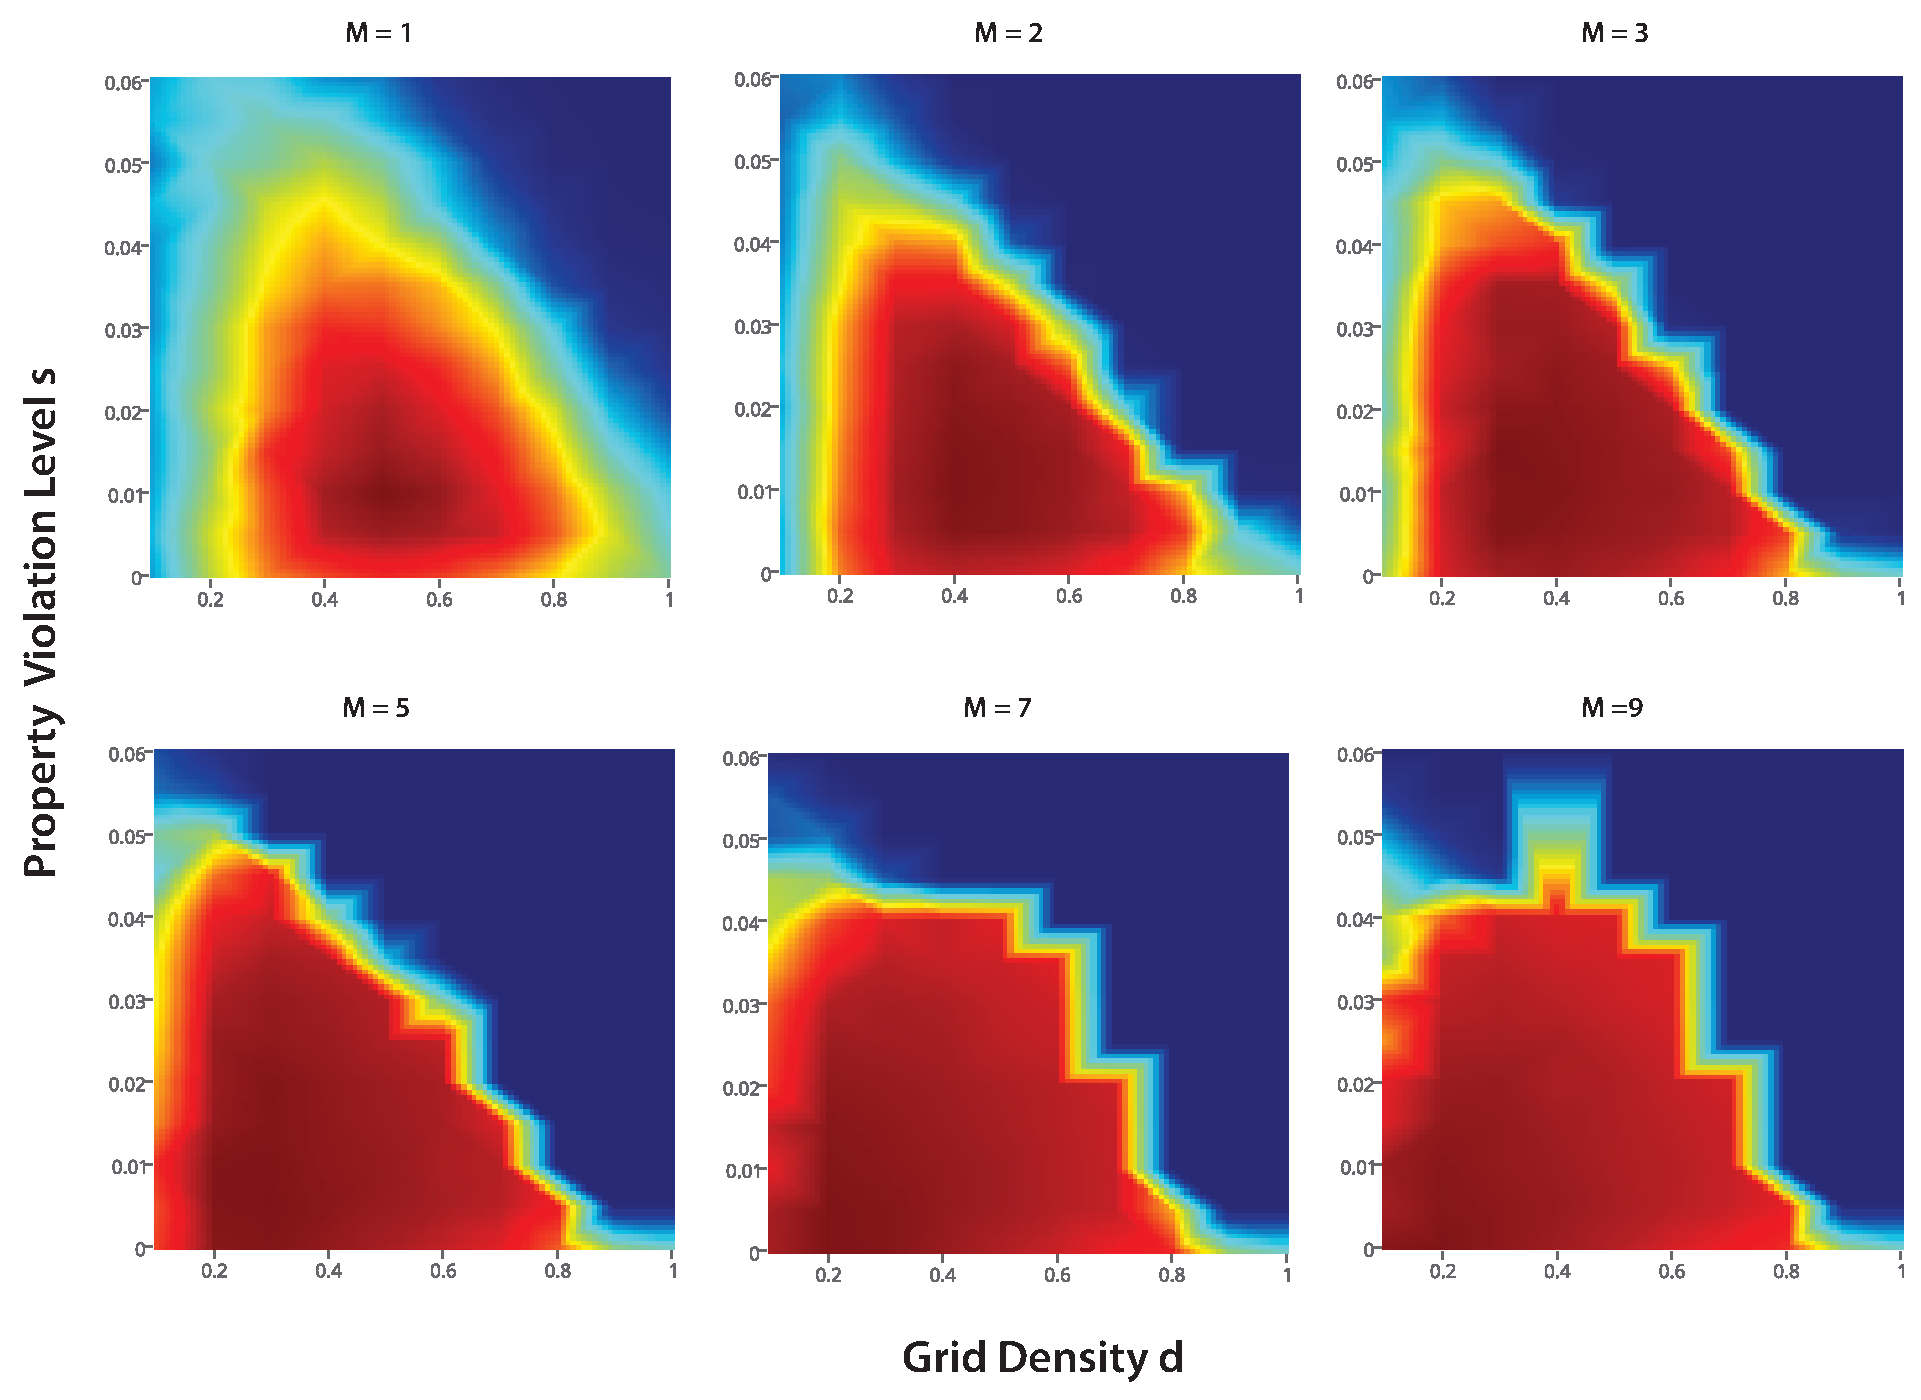
\includegraphics[width=14cm]{../figures2/heatmaps.eps}}
\caption{Cooperation levels after $N=200$ iterations [i.e., $200 \times 49^2 = 480,200$ Monte Carlo Steps (MCS)] for migration Moore's distances $M = \{1,2,3,5,7,9,11,15,20 \}$, as a function of population density $d$ and probability of property violation $s$. At initialization ($t=0$), there is a $50\%$ chance that a player will cooperate (resp. defect). The uneven landscapes reflect the statistical fluctuations of simulations. For all values of $M$, the cooperation exhibits a sharp drop for $d > d^*$  and $s > s^*$ with $(d^*,s^*)$ being a function of $M$. For high grid density ($d > 0.9$), cooperation cannot be sustained even with low property violation. As the migration range gets large $M > 9$ , the area of sustainable cooperation shrinks drastically.%(see SI Section \ref{SI:d09} for further details on {\it migration} and {\it property} games in densely populated worlds).
}
\label{fig:heatmaps}
\end{center}
\end{figure}


\begin{figure}[h]
\begin{center}
\centerline{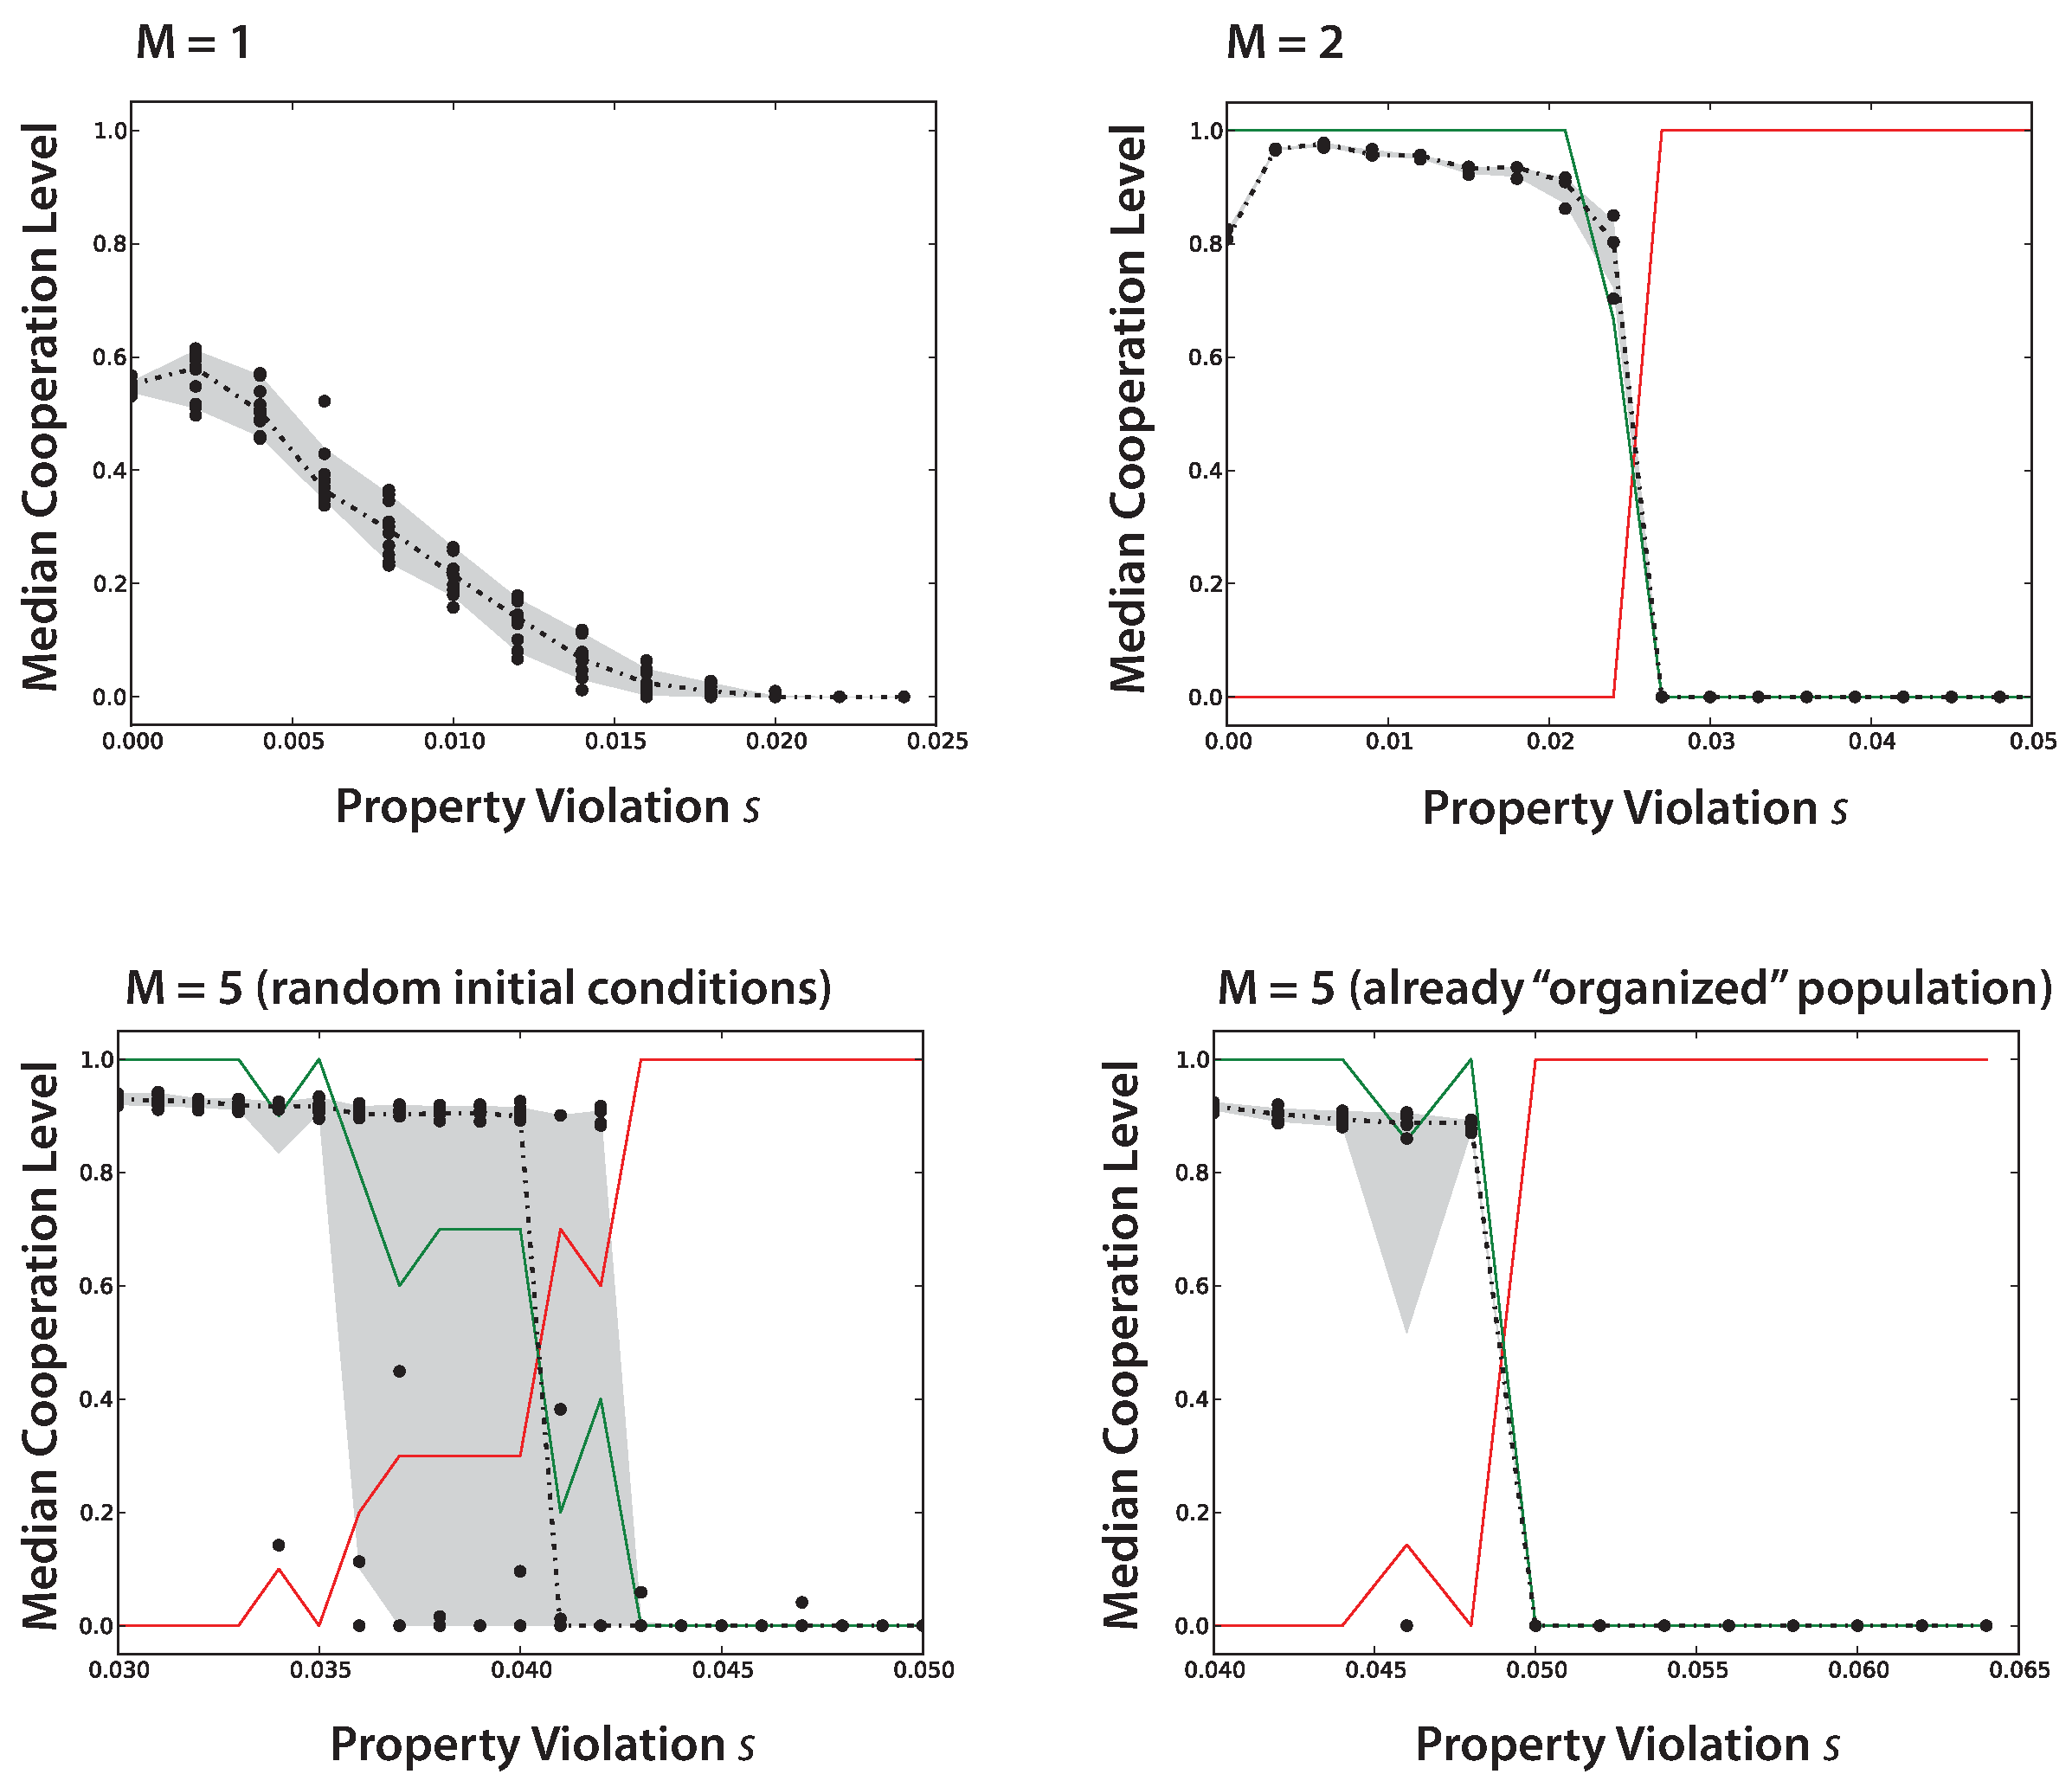
\includegraphics[width=9cm]{../figures2/phase_transitions.eps}}
\caption{Phase transition of cooperation levels for migration Moore's distances $M = \{1,2,5\}$ and population density $d=0.5$. {\bf a.} For $M=1$, the level of cooperation goes hardly above $0.6$ for property violation $s = 0.02$ and decreases to reach $0$ for $s > 0.02$ (actually, it takes a large number of iterations ($\approx 5000$) to converge to small values of cooperation for $s$ close but smaller than $0.02$, and it's not even sure cooperation $\rightarrow 0$ for $N \rightarrow \infty$). {\bf b.} For $M=2$, a sharp transition unfolds around $s^{*} = 0.025$ beyond which cooperation cannot survive. Comparison with$M=1$, shows the positive effects of larger migration ranges on cooperation. {\bf c.} For $M=5$, the transition point $s^{*}$ with equal probability that cooperative players will strive or disappear is $\approx 4.01\times10^{-2}$.  However, for $0.035 < s < 0.044$, cooperation can either be sustained or disappear, yet with decreasing (green line) or respectively increasing (red line) probabilities. The cooperation level after $N$ iterations is stochastic and does not depend on the initial grid configuration. {\bf d.}  Phase transition for $M=5$, given that cooperation clusters were already formed (property violation $s =0.042$ and cooperation level $c>0.09$: We search the new transition point $s^{*}$ beyond which cooperation disappears with non-random and already successful grid, with the aim to measure the resistance of an already established cooperative population The resistance of such already ``organized" population to property violation is $20\%$ higher than a population of cooperators initially randomly distributed across the grid.}
\label{fig:phase_transition}
\end{center}
\end{figure}



\begin{figure}[h]
\begin{center}
\centerline{\includegraphics[width=15cm]{../figures2/tseries_transition_dPayoff_M5_d05.eps}}
\caption{Payoff differences over time from property violation (blue), forced migration following property violation (green), success-driven migration (red), and strategy update (cyan). The top panels show sustained cooperation and $s = \{0.03,0.037,0.042,\}$ resp. outside, at lower and higher limits of the transition range (c.f., Figure \ref{fig:phase_transition}{\bf c}) for $M=5$: In all these case, a dynamic equilibrium is reached quickly and high levels of cooperation ($c > 0.9$). The bottom panels show the unstainable dynamics for same values of property violation at the edge of the phase transition range $s = \{0.037,0.042\}$ and for $s = 0.05$. What makes a difference between sustainable and unsustainable dynamics seems to be related to how fast the delta payoff from property violation can be reduced to a level ( $<2$) at which the combined (positive) effects of migration and strategy update seem to offset the negative effects of property violation. If this dynamic equilibrium is not met, the payoff resulting from strategy updates increases, reflecting the increased adoption of {\it defector} strategies. As a result, property violation does not payoff anymore, leading to unsustainable dynamics and collapse of cooperation.}
\label{fig:tseries}
\end{center}
\end{figure}


%\begin{figure}[h]
%\begin{center}
%\centerline{\includegraphics[width=9cm]{../figures/configurations_t200.eps}}
%\caption{Grid configurations at $t=200$, with fully rational agents (probability of imitation $m=1$), and grid density $d=0.5$. When there is no migration $M=0$ (and {\it a fortiori} no property violation $s=0$) (see {\it A.}), clusters of cooperators can only form by local influence, and the simulation is quickly frozen. As the migration range increases, larger clusters form when cooperators (see {\it B.,E.}) or defectors (see {\it D.,G.}) win. At the lower limit of the phase transition point $s \rightarrow s^{*}_{-}$, cooperators form clusters, which stay strong (large?) enough to keep defectors at bay (see {\it C.,F.}). When $s > s^{*}_{+}$ cooperation cannot survive. However, with larger migration range $M=5$, the transition point $s^*$ is almost three times larger, compared to $M=1$.}
%\label{fig:configurations_t200}
%\end{center}
%\end{figure}
%
%
%\begin{figure}[h]
%\begin{center}
%\centerline{\includegraphics[width=11cm]{../figures/configurations_t200_M11plus.eps}}
%\caption{Grid configurations at $t=200$, with fully rational agents (probability of imitation $m=1$), and grid density $d=0.5$ in the case of large migration ranges ($M = \{11,13\}$). For $M$ large enough, two distinct transition points appear ($s^{*}_{-}$ and $s^{*}_{+}$), with an intermediary stable state (see {\it C.} and {\it G.}), where cooperators are in minority ($c = 0.45\pm0.05$), yet their clusters resistant to defector invasions. Note that configurations look the same for $M=11$ and $M=13$, but the transition interval $(s^{*}_{-}$,$s^{*}_{+}$ has slightly larger values in the latter case, suggesting that populations with larger migration range can sustain more property violation.}
%\label{fig:configurations_t200_M11plus}
%\end{center}
%\end{figure}


%\begin{figure}[h]
%\begin{center}
%\centerline{\includegraphics[width=11cm]{../figures/configurations_t200.eps}}
%\caption{Grid configurations at $t=200$, with fully rational agents (probability of imitation $m=1$), and grid density $d=0.5$. When no migration (and {\it a fortiori} no property violation) is present (see {\it A.}), clusters of cooperators can only form by local influence, and the simulation is quickly frozen. As the migration range increases,  larger clusters form when cooperators (see {\it B.,E.}) or defectors (see {\it D.,G.}) win. At the lower limit of the phase transition point $s \rightarrow s^{*}_{-}$, cooperators form clusters, which stay strong (large?) enough to keep defectors at bay (see {\it C.,F.}).}\label{fig:comparison_no_with_migration}
%\end{center}
%\end{figure}




%\begin{figure}[h]
%\begin{center}
%\centerline{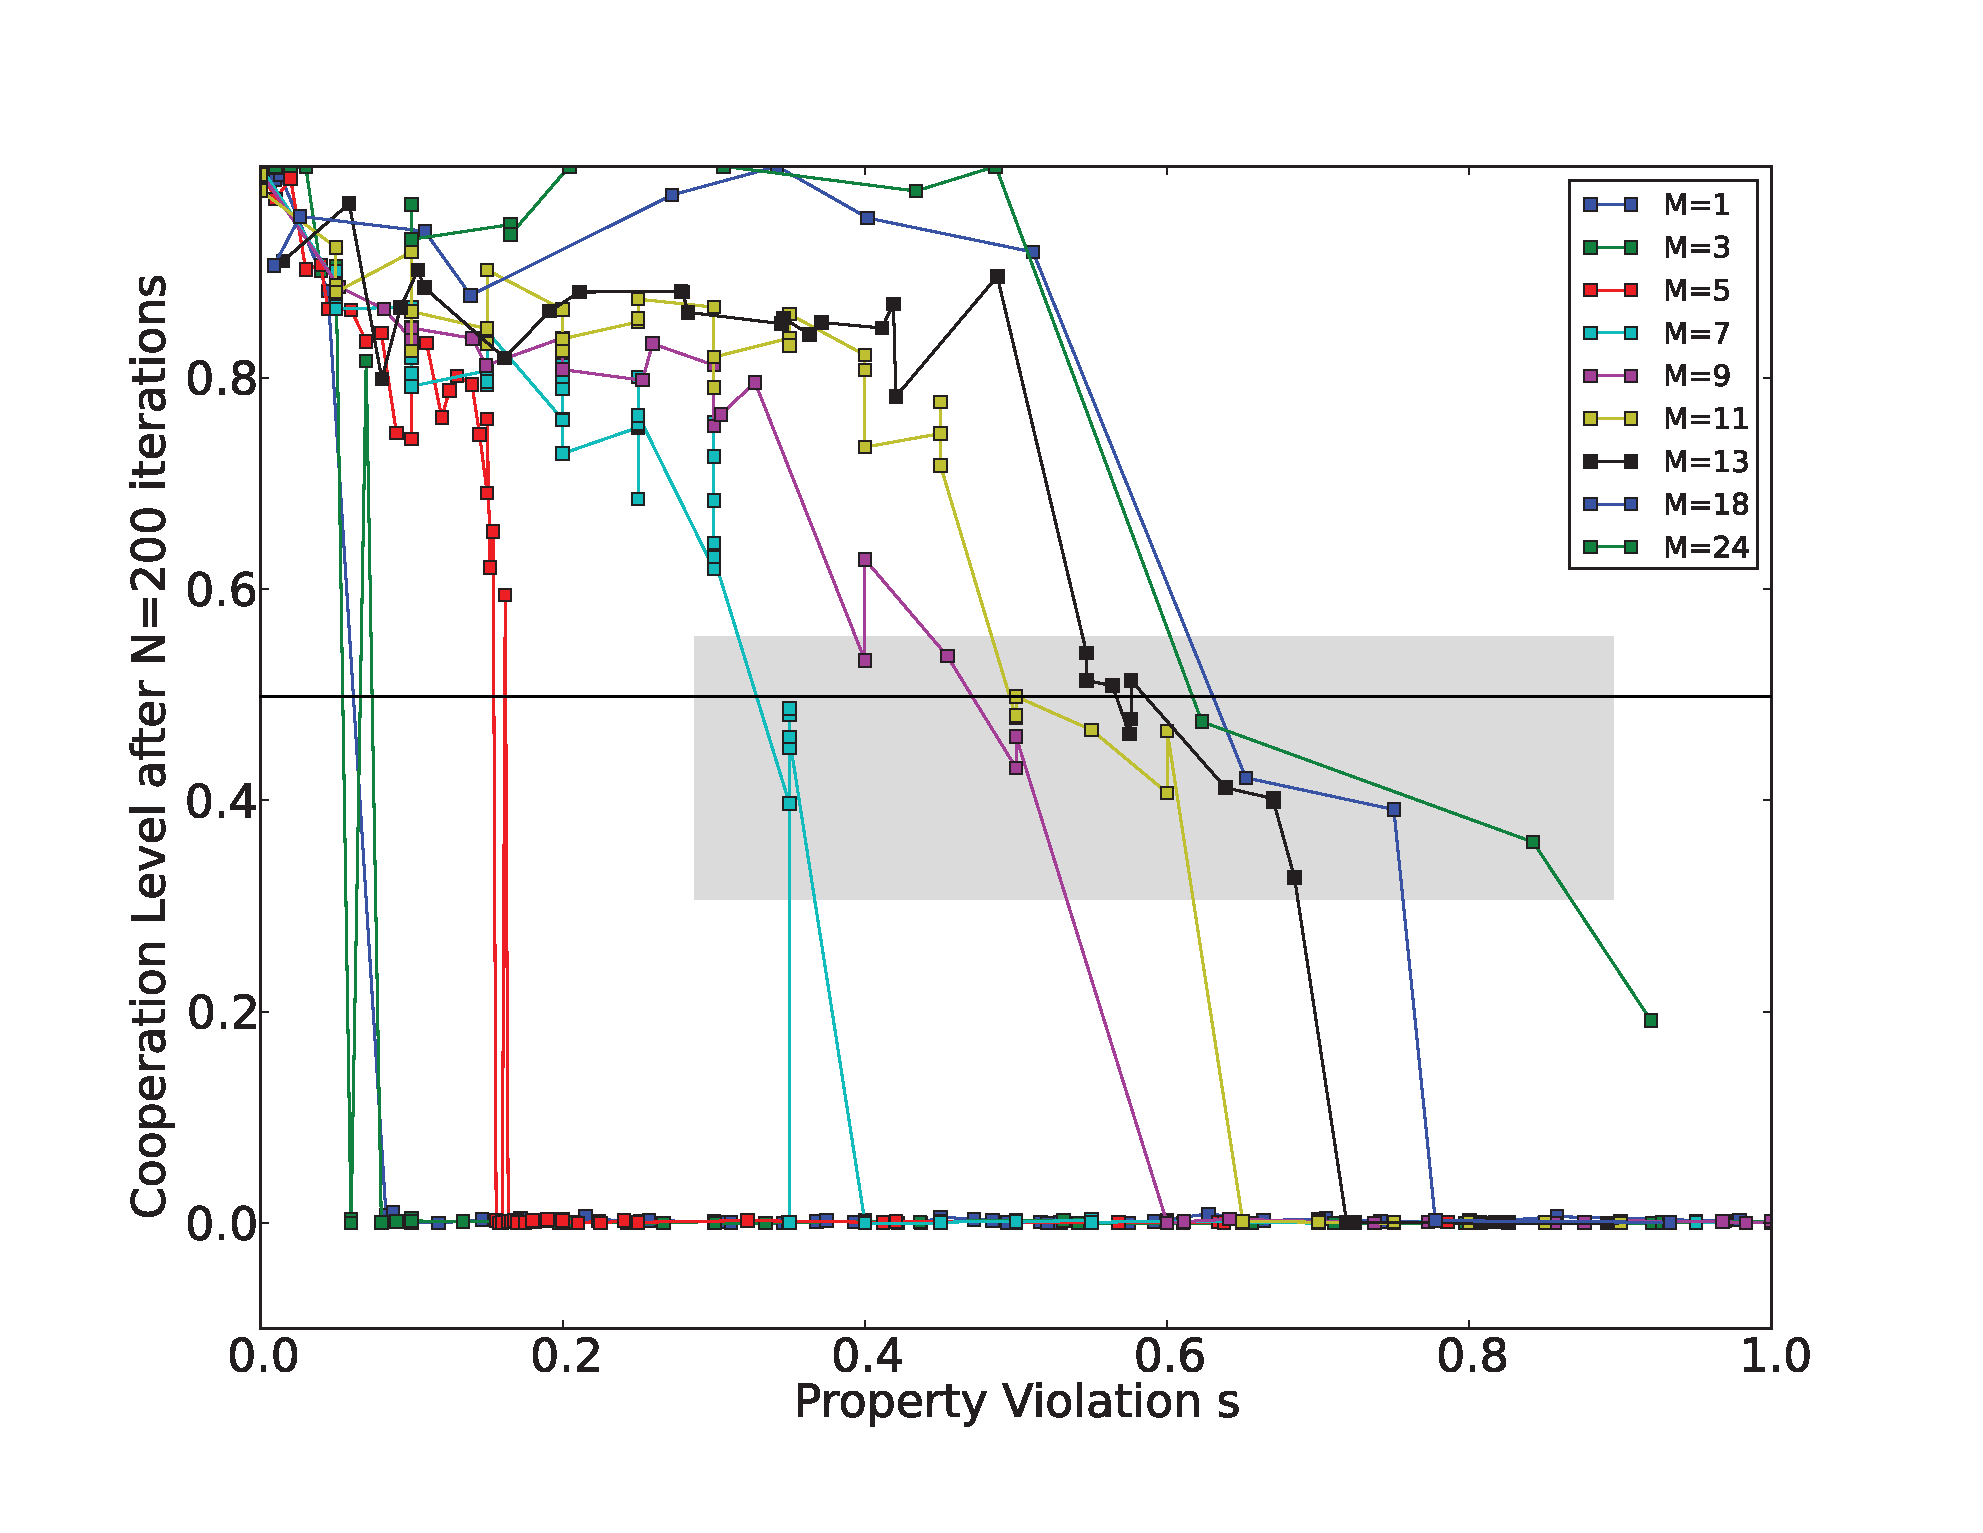
\includegraphics[width=15cm]{../figures/phase_transitions_2.eps}}
%\caption{Typical phase transitions for migration ranges $1 \leqslant M \leqslant 24$ ($0.4 \leqslant d < 0.6$). When there is no property violation $s = 0$, cooperators invade the world for any migration range $M > 0$. For small $M = \{ 1,3,5\}$, a sharp phase transition occurs at a transition point $s^{*}$, from a high level of cooperators in the populations ($c > 0.6$) when $s < s^{*}$ to entire collapse of cooperators for $s > s^{*}$. For $M \leqslant 5$, there is no intermediary state, whereas for $M \geqslant 7$, an intermediary state appears defined by $s^{*}_{-} < s < s^{*}_{+}$, with populations of cooperators in minority ($c \approx 0.45 < 0.5$) compared to defectors. For $M= \{ 7,9\}$, there is a non-zero probability of cooperation collapse, while for larger migration ranges ($M \geqslant 11$), this intermediary state becomes more stable, i.e., process converges almost surely  {\bf [to be further checked]}. Larger migration ranges increase both the maximum number of cooperators when $0 < s < s^{*}_{-}$, increase the lower $s^{*}_{-}$ and higher $s^{*}_{+}$ bounds of property violations, below (resp. above) which cooperative populations win (resp. disappear), and decreases the minimum average proportion of cooperative populations needed in order for cooperation to strive {\bf [to be further checked]}.}
%\label{fig:phase_transition}
%\end{center}
%\end{figure}








%
%
%\begin{figure}[h]
%\begin{center}
%%\centerline{\includegraphics[width=12cm]{Figures/CCDF_A.eps}}
%\caption{Representative spatial organizations for the {\it property game}: {\bf a.} Cooperation can be maintained despite 20\% of property violation probability $(M,d,s) = (9,0.5,0.2)$, {\bf b.} Cooperation collapses quickly for $s>s^*$  $(M,d,s) = (5,0.5,0.5)$, {\bf c.} and {\bf d.} phase transition at $s^{*} = 0.155\pm0.5$ and cooperation can be maintained or on the contrary collapse {\bf [discuss how it may be only a question of time before collapse $\rightarrow$ further simulations + stochastic considerations?]}, {\bf e.} Considerations for $(M,d,s) = (1, 0^+,0.5)$ (c.f. upper left panel Figure \ref{fig:cooperation_M}), and {\bf f.} Considerations for $(M,d,s) = (7,0.9,0^+)$.}
%\label{fig:configurations}
%\end{center}
%\end{figure}

